\begin{itemize}
	      	      
	\item \textbf{Scikit-learn}\\
        Scikit-learn, often abbreviated as Sklearn, includes a sub-module known as 'manifold', which is widely recognized for offering a comprehensive open-source implementation of various manifold learning algorithms. This Python package is primarily focused on user-friendliness. Although Scikit-learn includes algorithms aimed at scalability, its manifold learning techniques do not fall into this category. The methods provided in the manifold sub-module are not capable of processing out-of-core data, making it challenging to scale these methods for large datasets. Additionally, these methods face limitations in sharing intermediate results, such as eigenvector computations, between different algorithms. This can lead to inefficiencies during the data exploration process. To address these limitations, the Megaman package was developed.

        In our study, we utilized the Spectral Embedding functionality from the scikit-learn package to conduct experiments on 2 datasets in different conditions, which are elaborated upon as follows.\\
        \begin{itemize}
            \item \textbf{Sklearn Spectral Embedding on Swiss Roll dataset (10k points):} \\ 
            In our exploration of dimensionality reduction techniques using the scikit-learn package, we encountered a formidable obstacle due to the sheer volume of our data. Initially, we generated a Swiss roll dataset with 100,000 samples, aiming to apply Spectral Embedding, a sophisticated method for reducing data dimensions. Aware of the computational challenges posed by such a large dataset, we initially considered minibatch learning as a potential solution. Minibatch learning is an effective strategy for handling vast datasets by dividing them into smaller, more manageable batches. This method proves invaluable when dealing with datasets too large for the available computer memory, facilitating efficient use of limited memory resources.

            However, the nature of Spectral Embedding necessitates a different approach. Unlike methods that can be adapted to minibatch learning, Spectral Embedding requires a comprehensive analysis of the dataset's overall structure. It computes eigenvectors and eigenvalues from the Laplacian matrix, capturing the connectivity and similarities among data points. This computation demands simultaneous access to the entire dataset to ensure accurate embedding outcomes, as it hinges on a holistic understanding of the data's global interactions.

            To address the computational demands of processing the full dataset of 100,000 points with standard hardware, such as a computer with 12.7GB of RAM, we introduced an affinity condition based on the concept of nearest neighbors. We opted to limit our affinity calculations to the 40 nearest neighbors for each data point, a decision aimed at managing computational load while preserving the integrity of local neighborhoods essential for effective Spectral Embedding. This approach significantly reduces computational requirements by focusing on local structures, thereby making the process feasible on normal hardware without sacrificing the quality of the dimensionality reduction.

            Applying the 40-nearest-neighbors condition uniformly across analyses of both the 10,000- and 100,000-point datasets, we endeavored to ensure consistency in our experimental setup. This strategy was crucial for effectively reducing the computational burden, focusing on local point interactions, and excluding less relevant distant points. It allowed us to conduct our analysis within the memory constraints of standard computing resources while maintaining the local neighborhood's integrity, which is critical for the successful application of Spectral Embedding on large datasets. This approach underscores the challenges and innovative solutions required when dealing with large-scale data in the realm of dimensionality reduction.
            
                \begin{figure}[H]
                    \centering
                    \begin{subfigure}{0.45\textwidth}
                        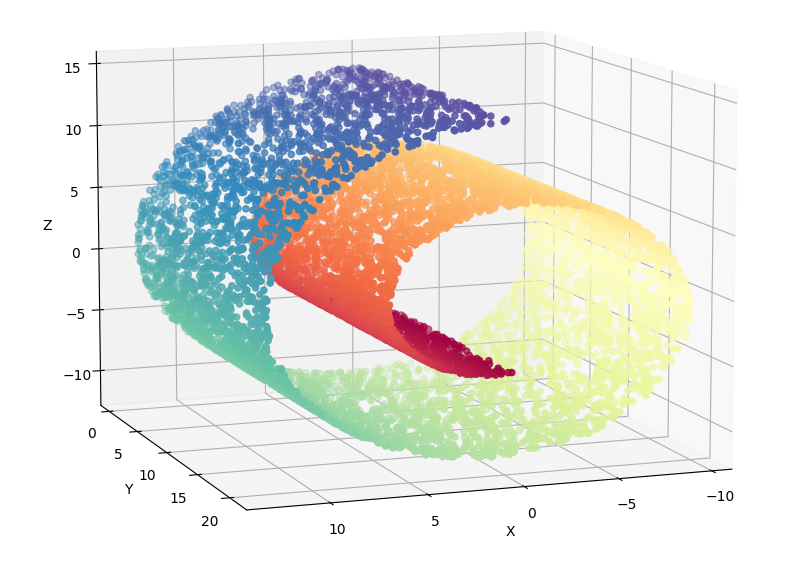
\includegraphics[width=\linewidth]{images/sklearn (2).png}
                        \caption{Swiss roll sampled 10k points}
                        \label{fig:sklearn_SwissRoll_10k}
                    \end{subfigure}         
                    \begin{subfigure}{0.45\textwidth}
                        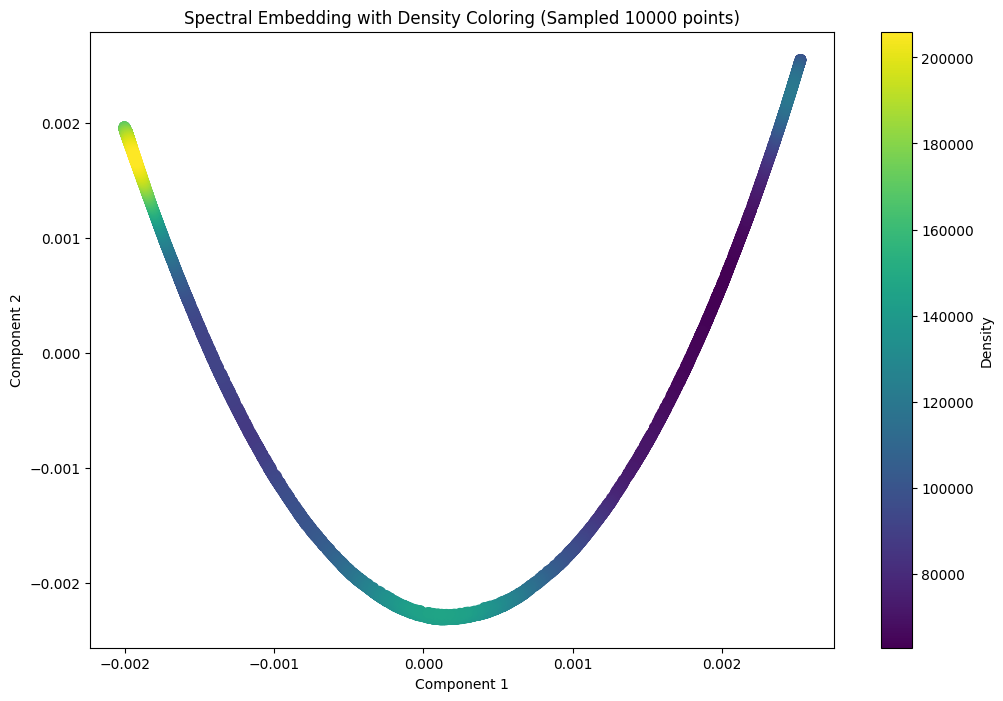
\includegraphics[width=\linewidth]{images/sklearn (4).png}
                        \caption{Spectral Embedding with density coloring Visualization of 10k point}
                        \label{fig:sklearn_SwissRoll_10k_R2}
                    \end{subfigure}
                    \caption{}
                    \label{fig:data_dol1}    	      	
                \end{figure}

            The scatter plot generated in Fig. \ref{fig:data_dol1} illustrates the application of Spectral Embedding on the Swiss roll data, with the aim of transforming it into a two-dimensional space. The primary objective of Spectral Embedding is to unfold the Swiss roll's manifold into a planar, two-dimensional representation, all the while maintaining the proximity of each point to its neighbors. The color scheme utilized in the plot mirrors that of the original three-dimensional visualization, denoting the original longitudinal position of each point on the manifold. The expectation from Spectral Embedding is the preservation of the color gradient in the 2D projection, which signifies that points adjacent to the manifold should ideally remain close in the reduced-dimensional space. However, the observed outcome did not align with this expectation, as the color gradient preservation—and consequently, the local neighborhood structure—was not as distinct as anticipated. This observation was further substantiated by a relatively low trustworthiness score of 0.4993, indicating that the embedding may not have effectively maintained the manifold's intrinsic geometric properties.
            
       
            \item \textbf{Sklearn Spectral Embedding on Swiss Roll dataset (100k points):}\\
            We expanded our dataset to include 100,000 points, as was explained above, presenting a significant challenge due to its size. Seen in subfigure \ref{fig:sklearn_SwissRoll_100k_R2}, the 'V' shaped plot indicates that the manifold has been unfolded. This representation is in a two-dimensional space where the x- and y-axes correspond to the two dimensions obtained from Spectral Embedding. The juxtaposition of these plots serves to illustrate the process of dimensionality reduction and how it can be visualized both before and after the application of Spectral Embedding. Also, it comes with density coloring which is especially useful for understanding how the points are distributed in the reduced space, offering insights into the underlying structure of the dataset that may not be immediately apparent from the raw Spectral Embedding alone.

                \begin{figure}[H]
                    \centering
                    \begin{subfigure}{0.45\textwidth}
                        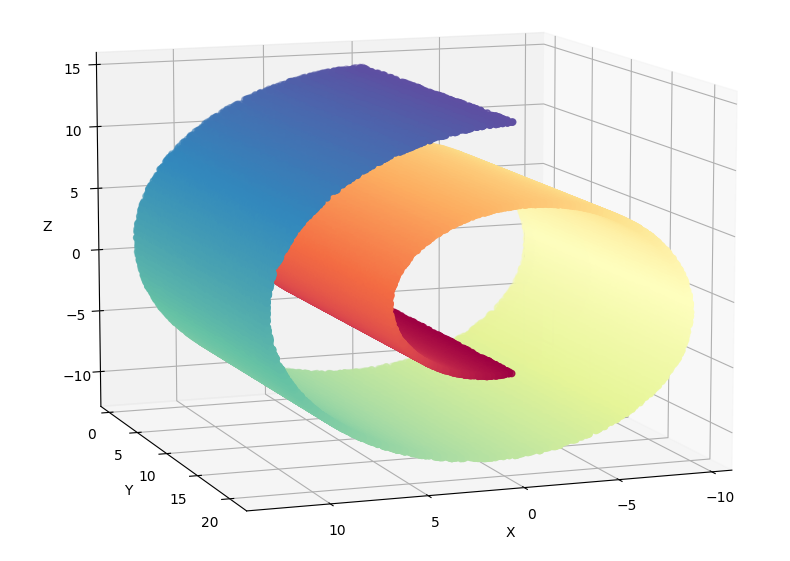
\includegraphics[width=\linewidth]{images/sklearn (5).png}
                        \caption{Swiss roll sampled 100k points}
                        \label{fig:sklearn_SwissRoll_100k}
                    \end{subfigure} 
                    \begin{subfigure}{0.45\textwidth}
                        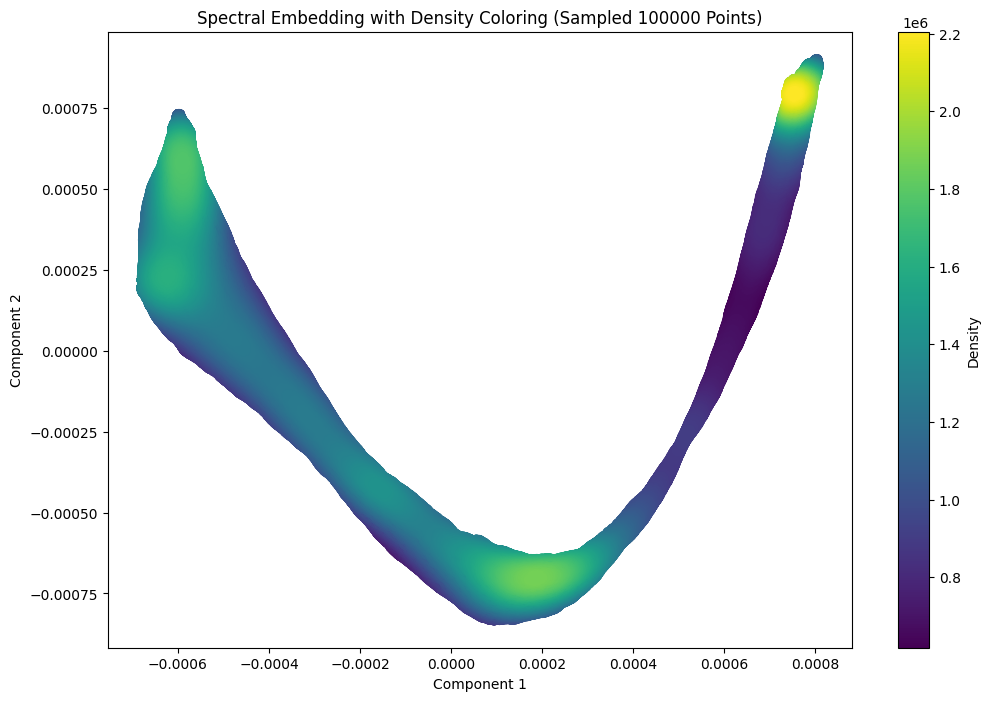
\includegraphics[width=\linewidth]{images/sklearn (7).png}
                        \caption{Spectral Embedding with density coloring Visualization of 10k point}
                        \label{fig:sklearn_SwissRoll_100k_R2}
                    \end{subfigure}
                    \caption{}
                    \label{fig:data_dol2}
               \end{figure}
           
            \item \textbf{Sklearn Spectral Embedding on Google News Word2Vec dataset (10k points):}
           
            We applied spectral embedding to real-world data using the Word2Vec model, which was pre-trained on Google News. This model represents words in its vocabulary as 300-dimensional vectors. For our analysis, we randomly selected a subset of 10,000 word vectors from the Word2Vec model, along with their corresponding vectors.

            The considerable size of the dataset posed a challenge, as it was too large to be processed in one fell swoop given memory limitations. To circumvent this, we turned to batch processing — an approach that, while not ideal, was chosen over other dimensionality reduction techniques like PCA due to its suitability to our specific constraints. This method involved dividing the dataset into manageable portions. For the 10,000 vector sample, we processed in batches of 1,000, which allowed us to perform the spectral embedding incrementally. When handling the more extensive 100,000 vector sample, we scaled the batch size up to 10,000. This strategic partitioning enabled the efficient transformation of high-dimensional word vectors into a lower-dimensional representation, ensuring the process remained manageable within the confines of our hardware's memory capabilities.
\\

            The data is embedded into 2 dimensions, and the result in Fig. \ref{fig:Spectral Embedding on Word2vec 10k points} shows a dense clustering of points in the center, suggesting that many word vectors are mapped close to each other in this reduced space. This could mean that a large number of words have similar contexts within the training corpus, leading to similar word vectors. Also, there are no clear, distinct clusters visible in the plot. In an ideal scenario, we might expect to see clusters of points that correspond to semantically similar words. The absence of such clusters might indicate that the Spectral Embedding has not effectively separated the words into distinct groupings based on their semantic relationships. It's also possible that the original high-dimensional space was very dense, and the Spectral Embedding is reflecting that density.
            
             \begin{figure}[H]
                  \centering
                  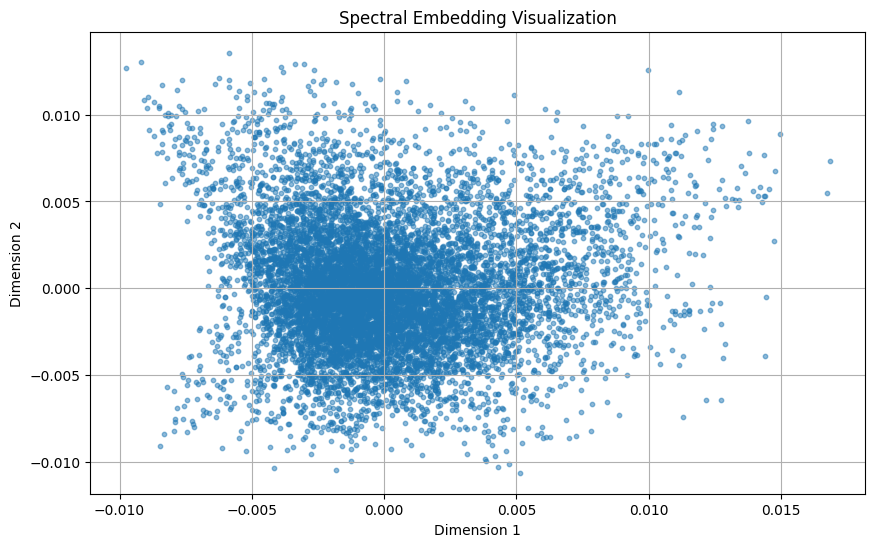
\includegraphics[width=0.5\textwidth]{images/sklearn (8).png}
                  \caption{Spectral Embedding on Word2vec 10k points}
                  \label{fig:Spectral Embedding on Word2vec 10k points}
              \end{figure}
	      
            
            \item \textbf{Sklearn Spectral Embedding on Google news Word2Vec dataset (100k points):}

            With a larger sample size, the visualization is more crowded, and the spread of the points is tighter. This could suggest a more accurate representation of the true relationships between words in the high-dimensional space, as more data points can lead to a better estimation of the true structure of the data.
            
             \begin{figure}[H]
                  \centering
                  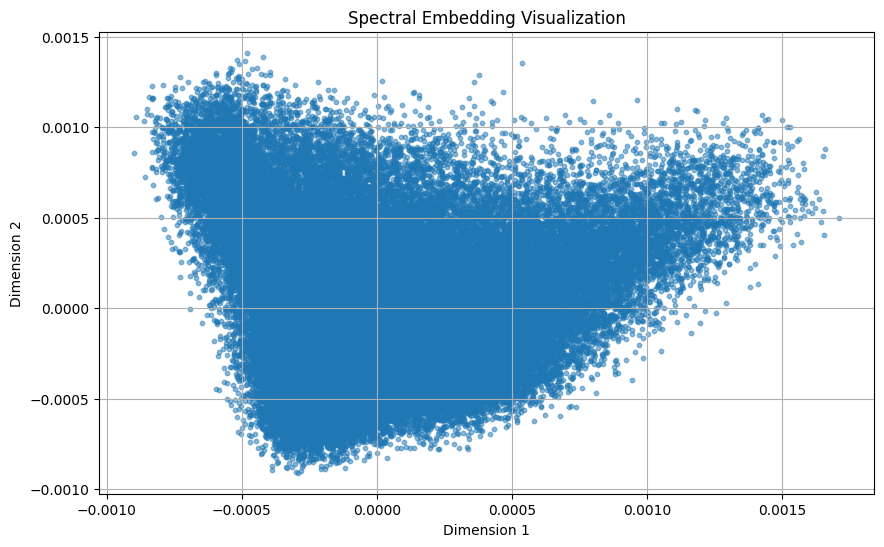
\includegraphics[width=0.5\textwidth]{images/sklearn (1).png}
                  \caption{Spectral Embedding on Word2vec 100k points}
                  \label{fig:Spectral Embedding on Word2vec 100k points}
              \end{figure}

            The resulting visualization for both samples seems to show a distribution of points in a dense, central band with fewer points as it radiates outward. This could indicate that many of the word vectors are similar to each other, forming a dense cluster in the center, while more unique or less frequent words are represented by points further away from the center.
	      
        \end{itemize}
	      	      
	      	      
	\item \textbf{Datafold Library}\\
	      One of the libraries that particularly helped us learn embeddings effectively was the datafold library. It is a Python package that provides data-driven models for point clouds to find an explicit manifold parametrization and to identify non-linear dynamical systems on these manifolds. Datafold provides us with an efficient implementation of the Diffusion Maps algorithm which we can use to learn embeddings on higher dimensional with large sizes too. The scalability factor provided by the datafold makes it a particularly useful choice for us to use on big datasets. We carried out multiple experiments with the library on our datasets which are discussed below.\cite{Datafold}
	      	      
	      \begin{itemize}
	      	\item \textbf{Datafold Diffusion maps for 10k points on Swiss Roll dataset:}\\
	      	      We start with a simple implementation of the diffusion maps on a moderately sized Swiss roll curve dataset consisting of 10k points. We first generate the dataset using sklearn's \textit{make\_swiss\_roll} function. One of the biggest challenges in applying diffusion maps is finding the optimal parameters. But, this becomes easy with datafold as it provides a function to find optimal parameters. We use the PCManifold \textit{optimize\_parameters} function to get the optimum value of the $\epsilon$ and \textit{cutoff} values.\\
	      	      Next, we use these parameters to fit on the Swiss roll curve dataset and compare potential two-dimensional embeddings. We can visually compare which eigenvectors provide us with the most information or in other words do the best job of unfolding the Swiss role curve into two-dimensional embedding space by plotting the first non-trivial eigenvector with other computed eigenvectors. Datafold also provides us with the option of automatic selection of embeddings via the \textit{LocalRegressionSelection} model. It tells us that the eigenvectors 1 and 5 are the best choice which can be seen in the figure \ref{fig:datafold_SwissRoll_10k}. We also get a very high trustworthiness score for our dataset which represents high quality embeddings.
	      	      \begin{figure}[H]
	      	      	\centering
	      	      	\begin{subfigure}{0.5\textwidth}
	      	      		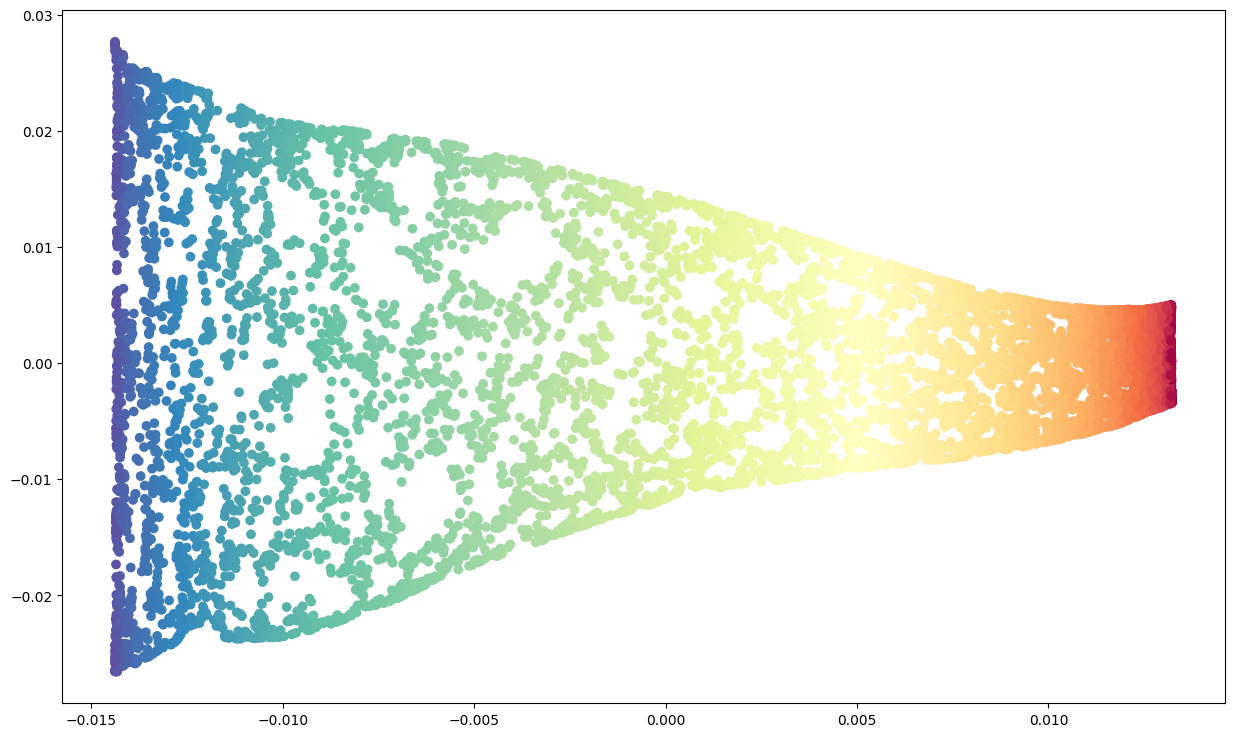
\includegraphics[width=\linewidth]{images/swiss_roll10k.png}
	      	      		\caption{10k points}
	      	      		\label{fig:datafold_SwissRoll_10k}
	      	      	\end{subfigure}
	      	      	\begin{subfigure}{0.5\textwidth}
	      	      		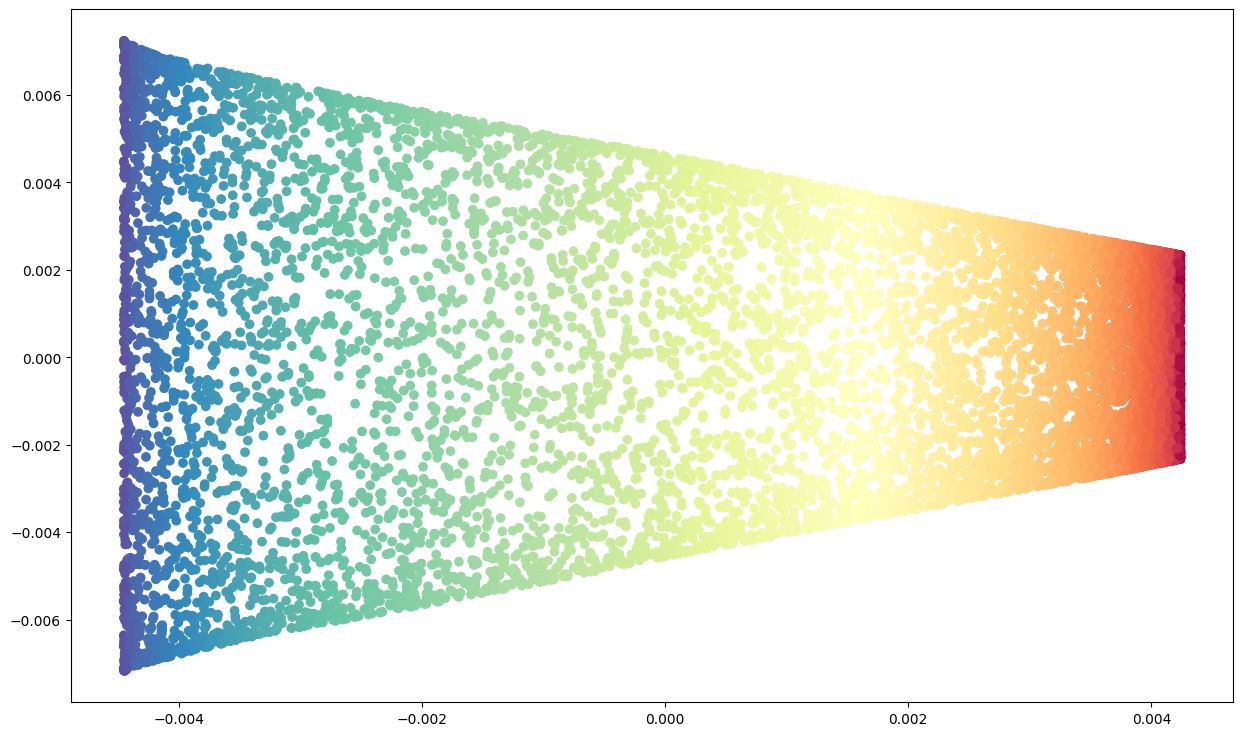
\includegraphics[width=\linewidth]{images/swiss_roll100k.png}
	      	      		\caption{100k points}
	      	      		\label{fig:datafold_SwissRoll_100k}
	      	      	\end{subfigure}
	      	      	\label{fig:data_dol}
	      	      	\caption{Datafold diffusion map results on Swiss roll dataset}
	      	      \end{figure}
	      	\item \textbf{Datafold Diffusion maps for 100k points on Swiss Roll dataset:}\\
	      	      Building upon our initial experiment, we escalated the complexity by increasing the number of points in the Swiss Roll Curve to 100,000. This expansion was aimed for us to test the scalability and robustness of the Datafold's diffusion maps algorithm. We mirrored the steps that we took for 10,000 points and fitted the diffusion maps models using the optimal parameters given by the PCManifold \textit{optimize\_parameters} function. The results can be seen in figure \ref{fig:datafold_SwissRoll_100k}. The trustworthiness score was also very high representing good embeddings.\\
	      	      Naturally, it took more time to compute the embeddings, but datafold was able to find it efficiently and quickly on our not so powerful computers while other libraries like Sklearn failed to do so without minibatching which might not even give particularly good results as discussed above.
	      	      
	      	\item \textbf{Datafold's Scalable Embedding via Landmark Diffusion on Swiss Roll dataset for 100k points:}\\
	      	      We get satisfactory results with the original implementation of datafold's diffusion map algorithm but it also exhibits a notable trade-off with computational time, especially when we increase the dataset size. It is also unable to deal with very large datasets: in our case, it couldn't handle a Swiss Roll curve with 1 million points. Fortunately, datafold offers us an alternative method that not only accelerates the embedding generation process but also extends the compatibility to substantially larger datasets.\\
	      	      This is done via the Roseland algorithm which can be viewed as a generalization of the diffusion map algorithm sharing various properties. The Roseland algorithm utilizes a "landmark set" which can be much smaller than the full dataset and employs this to calculate the affinity matrix. In particular, when constructing the transition probability matrix, which can be especially computationally intensive for large datasets, the Roseland algorithm doesn't use all of the data points but only a subset (which we referred to as the "landmark set"). This allows to reduce the computational complexity with the classical Diffusion Maps algorithm from $O(N^3)$ to $O(n^2N)$ or $O(n^3)$, where $N$ is the total number of data points and $n$ is the number of selected points for approximation. 
                    In the end, the datafold's implementation of the Roseland algorithm allows us to get faster results on the Swiss roll dataset with 100k points with comparable trustworthiness metrics while providing much faster results.\\
	      	      The steps involved in applying the Roseland algorithms are mostly the same with just an extra choice of selecting the landmark parameter. We tried different landmark parameters and found that a value of 0.4 gave pretty good results without compromising the computational time. While the diffusion map algorithm took somewhere close to 7 minutes to calculate the embeddings, the Roseland algorithm calculated in around 1 minute which is a big improvement in runtime. The results obtained by the Roseland algorithm can be seen in figure \ref{fig:datafold_SwissRollRoseland_100k}
	      	      
	      	      \begin{figure}[H]
	      	      	\centering
	      	      	\begin{subfigure}{0.5\textwidth}
	      	      		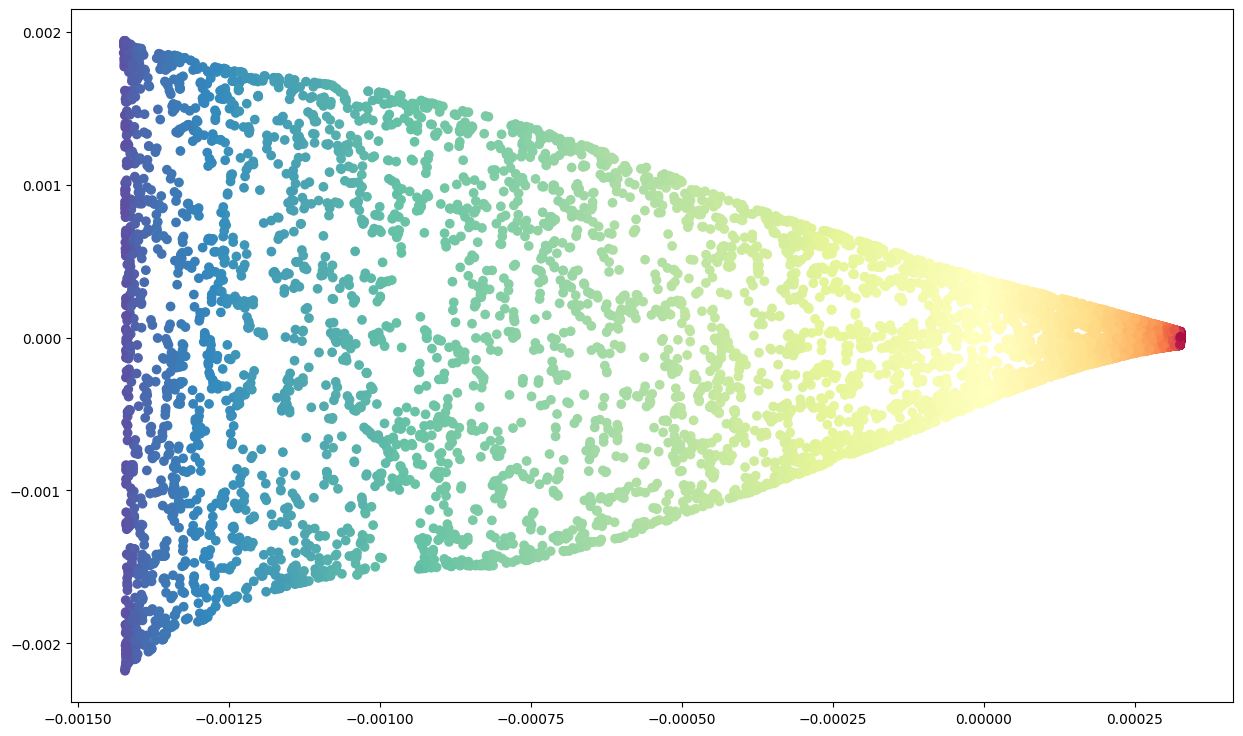
\includegraphics[width=\linewidth]{images/roseland_SwissRoll100k.png}
	      	      		\caption{100k points}
	      	      		\label{fig:datafold_SwissRollRoseland_100k}
	      	      	\end{subfigure}
	      	      	\begin{subfigure}{0.5\textwidth}
	      	      		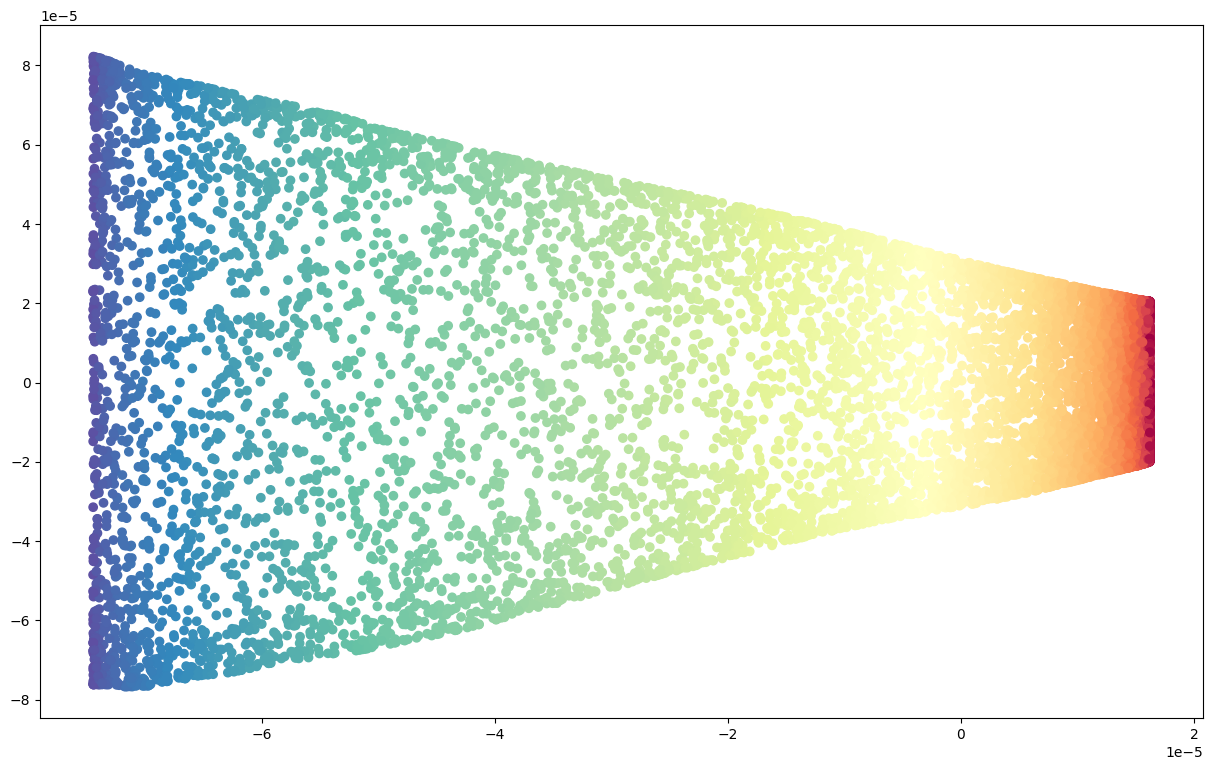
\includegraphics[width=\linewidth]{images/roseland_SwissRoll1million.png}
	      	      		\caption{1 million points}
	      	      		\label{fig:datafold_SwissRollRoseland_1M}
	      	      	\end{subfigure}
	      	      	\label{fig:roseland}
	      	      	\caption{Datafold Scalable Embedding via Landmark Diffusion}
	      	      \end{figure}
	      	      
	      	\item \textbf{Datafold's Scalable Embedding via Landmark Diffusion on Swiss Roll dataset for 1M points:}
	      	      Extending on our previous implementation using the Roseland algorithm\cite{Roseland}, we finally tried testing the library on 1 million points which has not been possible using the other libraries like sklearn and UMAP. But, to our surprise, with a landmark value of 0.2, we were able to generate the 2-dimensional embedding of the Swiss roll curve using Datafold's Roseland model. Although choosing a lower landmark value forces us to tradeoff between accuracy and computational runtime, it allows us to get meaningful results on our not so powerful computers. This is particularly exciting and is comparable to the Megaman package itself which allowed us to use the Spectral Embedding method on very large datasets. The result of the embeddings can be seen in the figure \ref{fig:datafold_SwissRollRoseland_1M}. Although it took us more than an hour and a half to calculate the embeddings, the possibility of calculating it is itself a big advantage.

              \item \textbf{Datafold Diffusion Maps on Google news Word2Vec dataset (10k points):}
              We also applied the original Diffusion Map model provided by datafold on the Word2Vec dataset. In order to run the algorithm, we had to tweak the parameters $\epsilon$ to a pretty low value of 0.1 as running it with a higher epsilon value or the optimal value suggested led to a memory error due to extensive internal calculations. Although we were able to apply the Diffusion Maps model, we couldn't get satisfactory results from it as can be seen in figure \ref{fig:datafold-word2Vec}. \\
              Several factors might be responsible for this outcome. First, there could be some issues with the preprocessing of the dataset, and it might need some refinement to improve the algorithm's performance on this specific dataset. Alternatively, the Diffusion Map algorithm may not be the best choice for dimensionality reduction in the context of the Word2Vec dataset. We might need to look at other algorithms capable of generating the embeddings for this dataset.
              \begin{figure}[H]
                  \centering
                  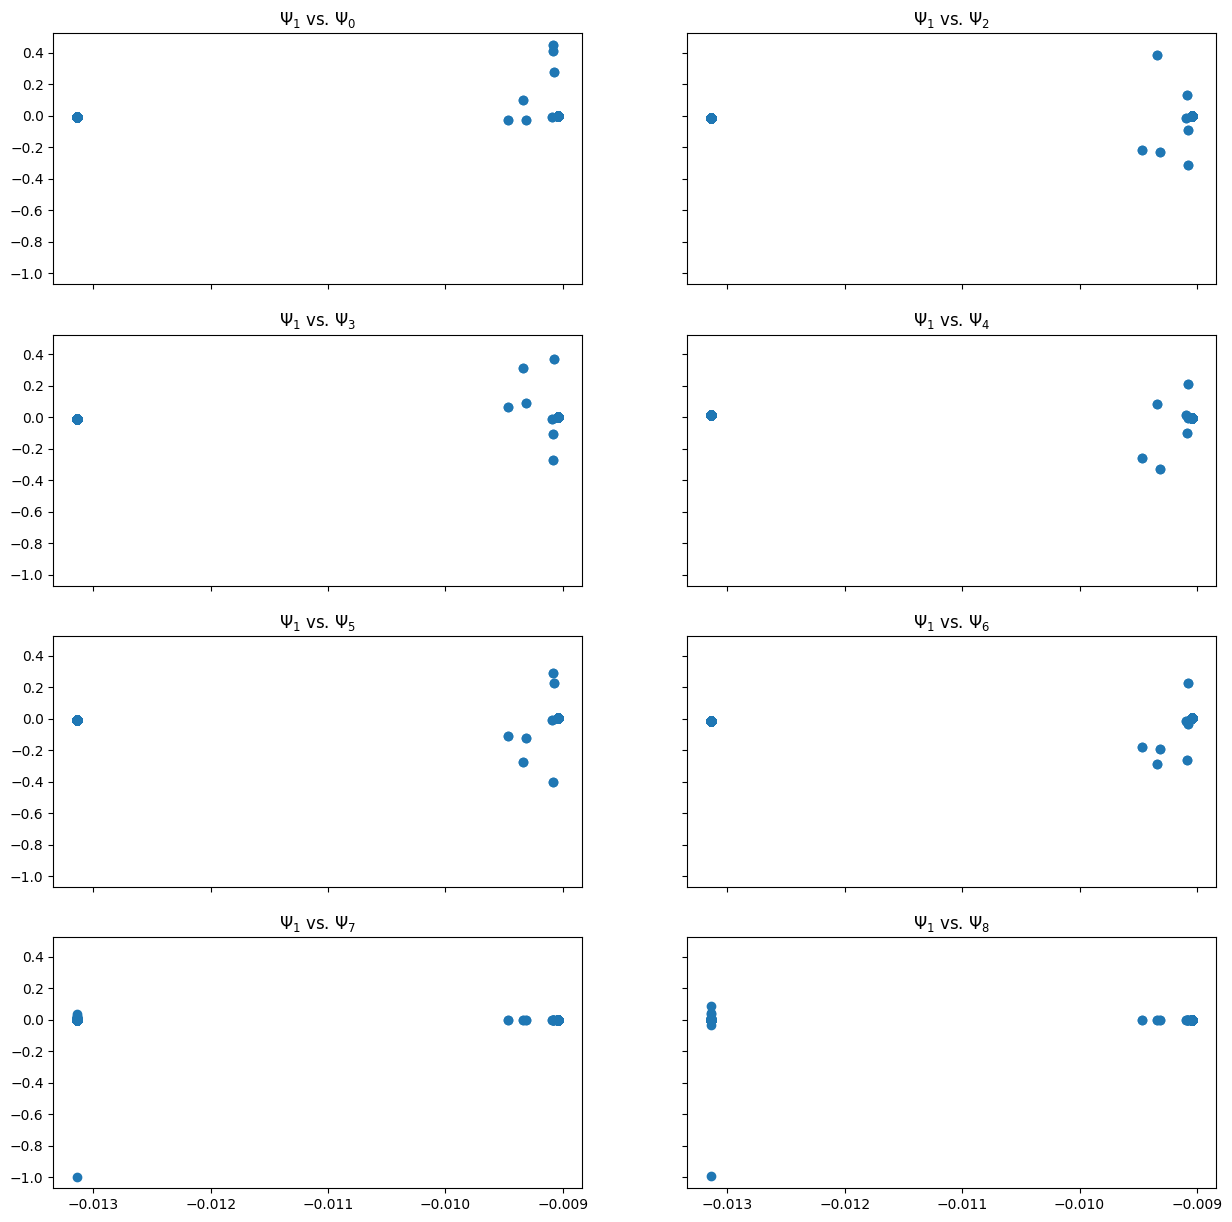
\includegraphics[width=0.5\textwidth]{images/datafold_output_word2vec.png}
                  \caption{Diffusion Map on Word2Vec}
                  \label{fig:datafold-word2Vec}
              \end{figure}
	      \end{itemize}

       \item \textbf{UMAP and NVIDIA's RAPIDS:}
	      	      
	      In our quest for high-speed data analysis, we discovered the power of Uniform Manifold Approximation and Projection (UMAP), a dimensionality reduction technique introduced in 2018 by McInnes et al.\cite{mcinnes2020umap} UMAP stands out due to its ability to preserve both local and global structures within data, providing a comprehensive representation of the original high-dimensional space. This is a significant improvement over techniques such as t-SNE (t-Distributed Stochastic Neighbor Embedding), which primarily focuses on local structure preservation. 
	      	      
	      UMAP operates by leveraging the concept of a manifold, a shape that resembles a flat Euclidean space when zoomed in. The algorithm constructs a weighted graph from the high-dimensional data, where each data point is a node, and edges are drawn between nodes that are close to each other in the high-dimensional space. The weight of each edge corresponds to the distance between the nodes it connects. This graph construction is based on the concept of a fuzzy simplicial set, a mathematical structure used to capture the topological features of the manifold. 
	      	      
	      Once the graph is constructed, UMAP seeks to find a lower-dimensional representation of the data that preserves the topological structure of the original high-dimensional data as much as possible. This is achieved by minimizing a function that measures the difference between the high-dimensional graph and the lower-dimensional representation using a variant of stochastic gradient descent. The result is a lower-dimensional representation of the data that maintains the essential topological features of the original high-dimensional data, making UMAP a powerful tool for visualizing and understanding complex datasets.
	      	      
	      To further enhance the efficiency of UMAP, we turned to NVIDIA’s RAPIDS library, an open-source suite of GPU-accelerated data science and AI libraries. Specifically, we utilized its cuML component, which provides a GPU-accelerated implementation of UMAP. This implementation leverages the parallel processing capabilities of the GPU, operating on a random sample of the full dataset for enhanced efficiency with larger datasets. 
	      	      
	      Built on NVIDIA CUDA-X AI, RAPIDS simplifies the complexities of GPU operations and data center communication protocols. It offers the flexibility to run anywhere—cloud or on-premises—and can scale from a workstation to multi-GPU servers to multi-node clusters. This combination of UMAP and NVIDIA's RAPIDS library presents a powerful and efficient solution for high-speed data analysis.\\

\textbf{ Experiments using Rapids' UMAP}

In our study, we conducted tests on two datasets: sklearn’s Swiss roll and a dataset provided by Google. Both datasets contain 10,000 and 100,000 data points. Despite our efforts to manage GPU memory efficiently, we encountered a bottleneck in memory capacity when attempting to increase the number of data points significantly. This limitation suggests that, despite its many advantages, UMAP may not be the optimal solution for our problem when dealing with extremely large datasets. Further research is needed to explore alternative methods or optimizations that can overcome this memory constraint. This finding underscores the importance of considering the specific requirements and constraints of a problem when selecting a dimensionality reduction technique.


\begin{itemize}
            \item \textbf{Dimensionality reduction on swiss roll dataset (10k points)}
        Our initial tests were conducted on a Swiss roll dataset comprising 10,000 points. As anticipated for a dataset of this size, the UMAP algorithm was executed swiftly. The accuracy of the dimensionality reduction was high, as evidenced by a trustworthiness rate of 0.9997. This result underscores the efficacy of UMAP in accurately reducing dimensions while maintaining the integrity of the data structure. [Figure \ref{fig:umap_swiss10k}]
        
         \item \textbf{Dimensionality reduction on swiss roll dataset (100k points)}
        To further evaluate the capabilities of UMAP, we expanded the dataset to 100,000 points. While there was a slight decrease in accuracy, the trustworthiness rate remained high, indicating that UMAP effectively handles larger datasets with minimal impact on performance. [Figure \ref{fig:umap_swiss100k}]

            \begin{figure}[H]
                \begin{subfigure}{0.5\textwidth}
                    \centering
                    \captionsetup{justification=centering}
                    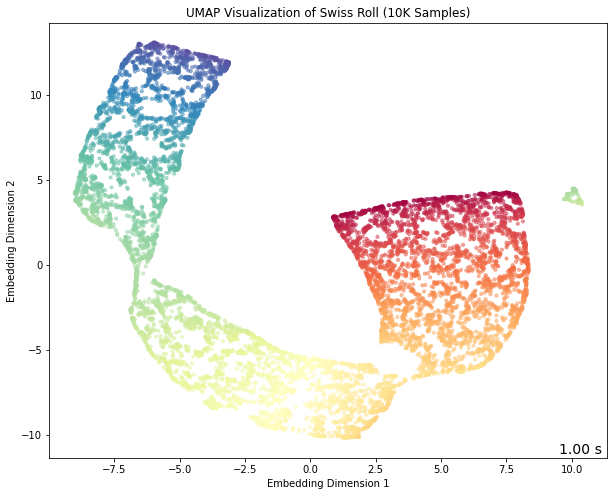
\includegraphics[width=\textwidth]{images/umap_swiss10k.png}
                    \caption{10K DataPoints}
                    \label{fig:umap_swiss10k}
                \end{subfigure}
                \begin{subfigure}{0.5\textwidth}
                    \centering
                    \captionsetup{justification=centering}
                    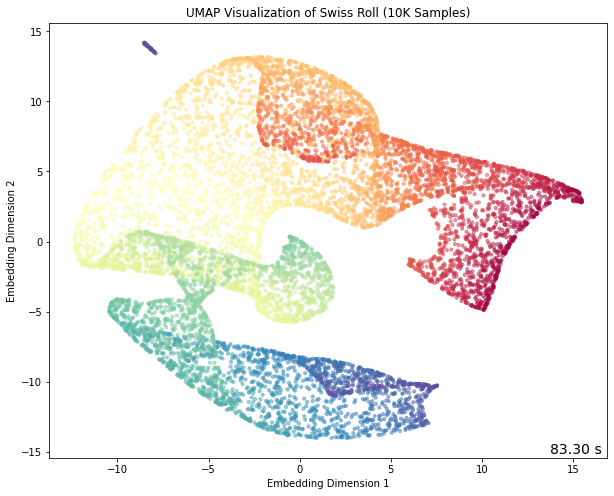
\includegraphics[width=\textwidth]{images/umap_swiss100k.png}
                    \caption{100K DataPoints (only random 10k shown)}
                    \label{fig:umap_swiss100k}
                \end{subfigure}
                \caption{UMAP SwissRoll}
                \label{fig:umap_swiss}
            \end{figure}

            \item \textbf{Dimensionality reduction on Google news Word2Vec dataset:}
            Our exploration extended to Google’s Word2Vec dataset, with tests conducted on both 10,000 [Figure \ref{fig:umap_word2vec10k}] and 100,000 [Figure \ref{fig:umap_word2vec100k}] data points. Interestingly, we observed a notable decrease in accuracy compared to the Swiss roll dataset for both cases. However, this reduction in accuracy was accompanied by an increase in computational speed. This suggests that while UMAP’s performance on the Word2Vec dataset was faster, it came at the cost of accuracy. This trade-off between speed and accuracy is a crucial aspect to consider in the context of large-scale, real-world applications.

            \begin{figure}[H]
                \begin{subfigure}{0.5\textwidth}
                    \centering
                    \captionsetup{justification=centering}
                    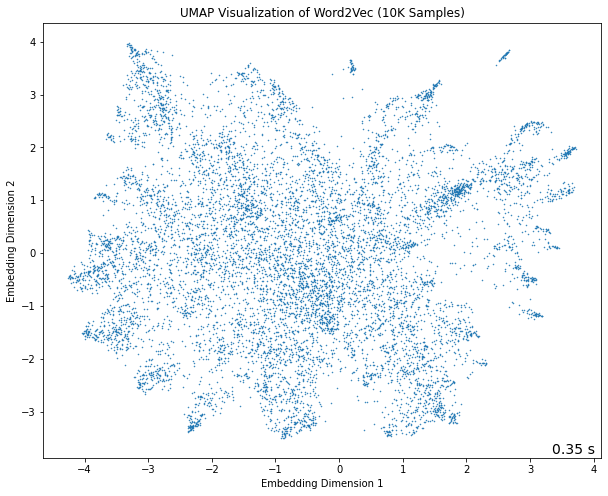
\includegraphics[width=\textwidth]{images/umap_word2vec10k.png}
                    \caption{10K DataPoints}
                    \label{fig:umap_word2vec10k}
                \end{subfigure}
                \begin{subfigure}{0.5\textwidth}
                    \centering
                    \captionsetup{justification=centering}
                    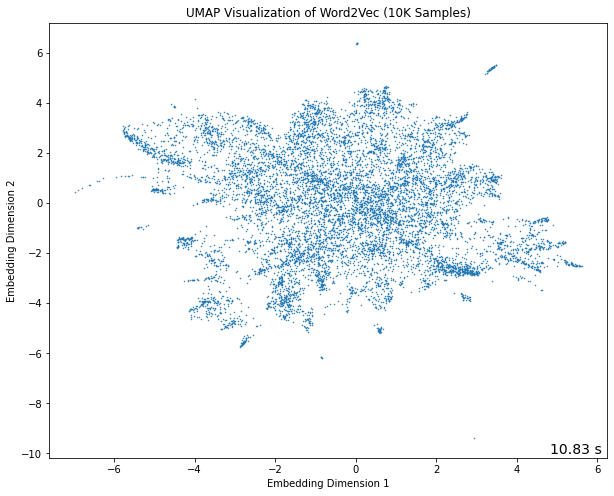
\includegraphics[width=\textwidth]{images/umap_word2vec100k.png}
                    \caption{100K DataPoints (only random 10k shown)}
                    \label{fig:umap_word2vec100k}
                \end{subfigure}
                \caption{UMAP Word2Vec}
                \label{fig:umap_word2vec}
            \end{figure}


    
\end{itemize}



       
	     
	      	      
	\item \textbf{Autoencoder based dimensionality reduction}\\
	      We also used an innovative approach utilising an autoencoder to reduce the dimensionality of our input features, yielding lower-dimensional embeddings on our datasets.\\
	      Autoencoders prove to be particularly advantageous in our context, excelling at capturing intricate non-linear relationships with the data. Throughout the training phase, the autoencoder dynamically learns to encode and decode the input features by establishing a compact latent representation. This lower-dimensional latent representation aims to capture the most salient and informative features of our datasets. After the completion of the training, we can extract the encoder component of the autoencoder. This extracted encoder serves as a dimensionality reduction tool providing us with reduced dimensional data that captures the most essential information of the input data.\\ \\
	      \textbf{Autoencoder architecture}\\ 
	      A simplified representation of our autoencoder architecture can be seen in figure \ref{fig:autoencoder-architecture}. It consists of multiple dense layers with varying numbers of neurons. The input layer receives the data. Following the input layer, we have a dense layer with 128 neurons, connected to a layer with 64 neurons and subsequently to a layer with 32 neurons. This final layer produces a 2-dimensional encoded representation, effectively capturing the essential features of our input data. \\
	      The decoder follows a mirrored architecture to reconstruct the original input from the latent representation. We also used Batch Normalization in the model to facilitate a smoother learning process. A comprehensive overview of the model structure can be seen in figure \ref{fig:autoencoder-summary}.\\ \\
	      
	      \begin{figure}[H]
	      	\centering
	      	\begin{subfigure}{0.5\textwidth}
	      		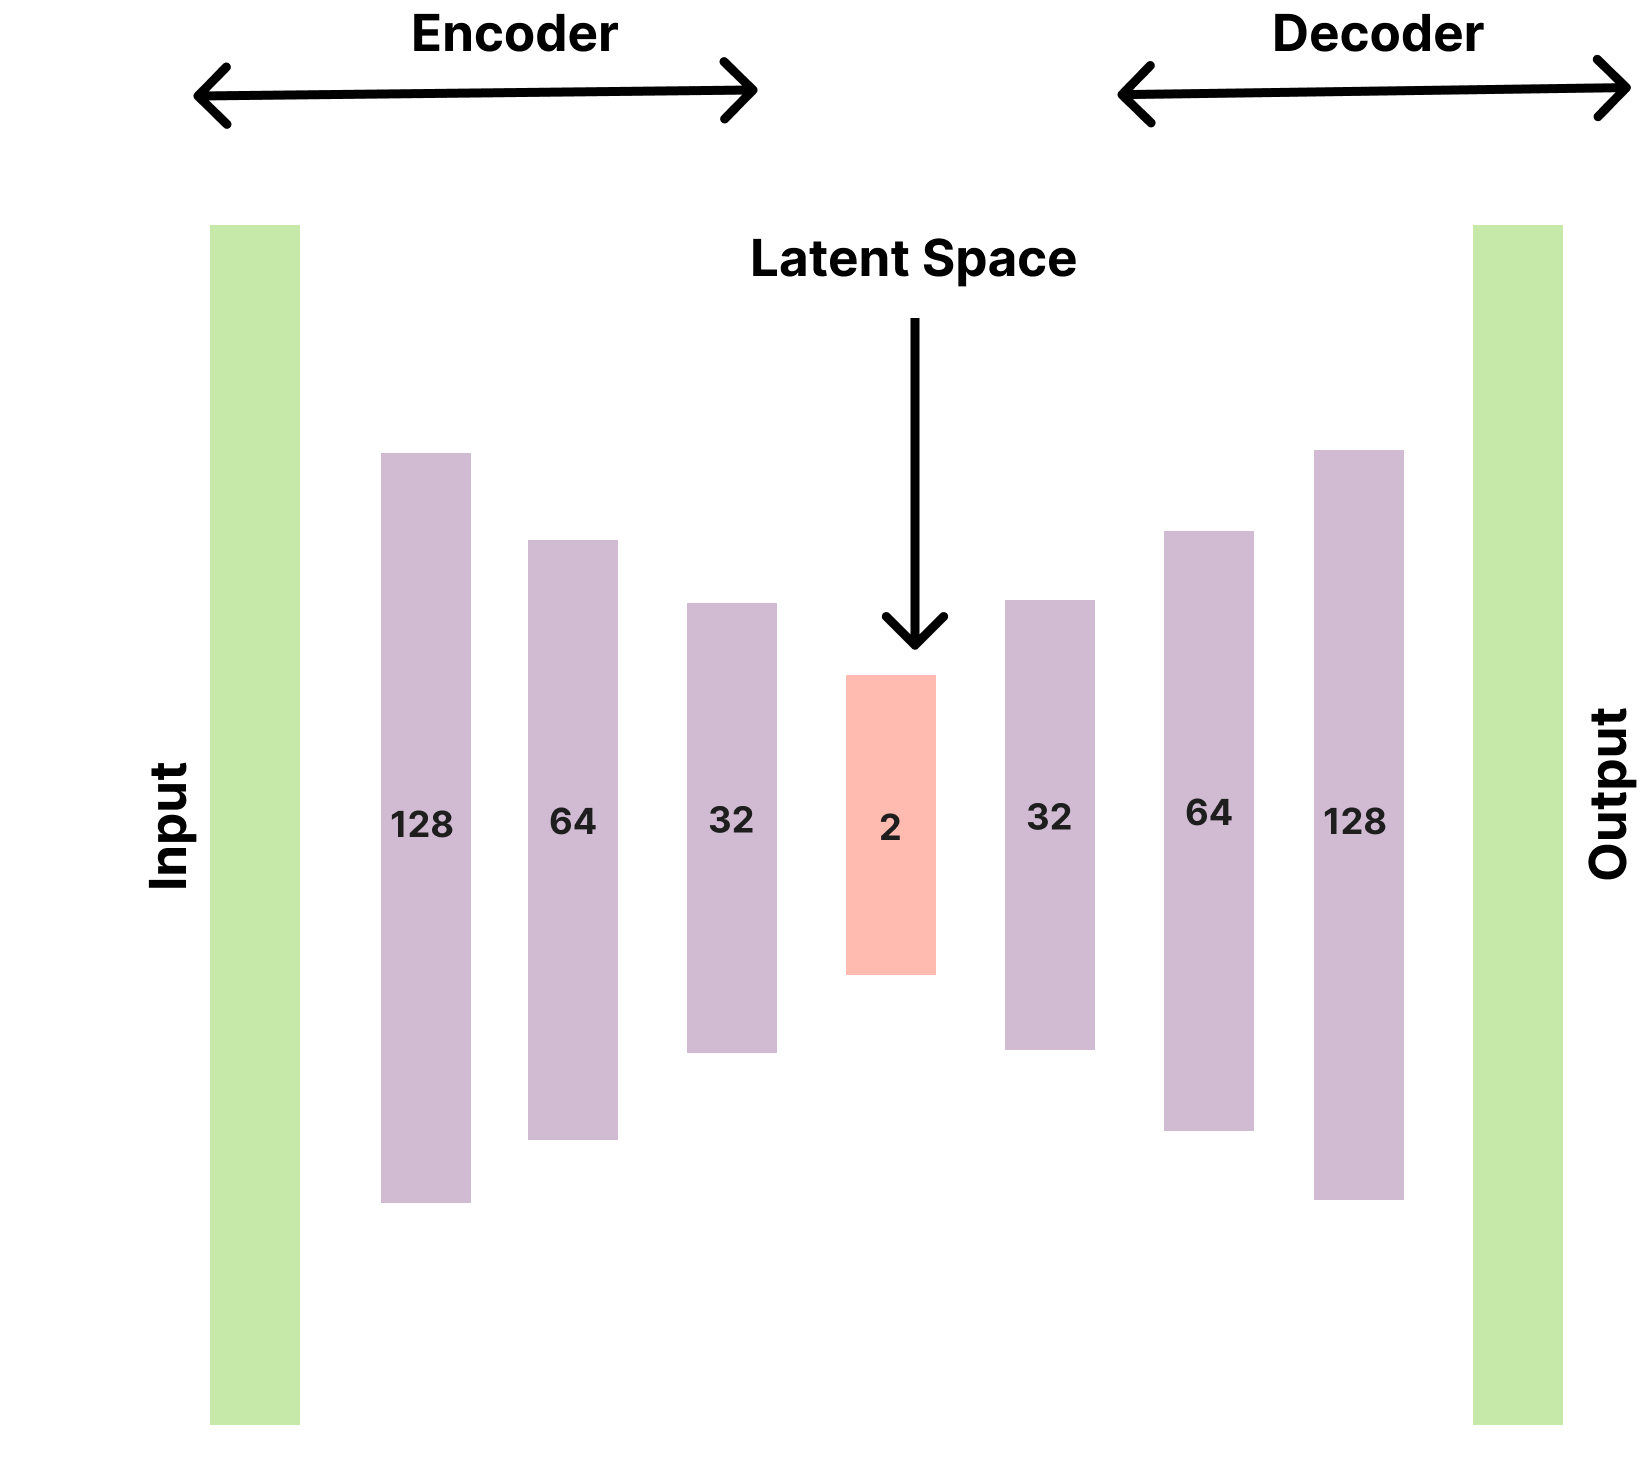
\includegraphics[width=\linewidth]{images/autoencoder_Architecture.png}
	      		\caption{Autoencoder architecture}
	      		\label{fig:autoencoder-architecture}
	      	\end{subfigure}
	      	\begin{subfigure}{0.5\textwidth}
	      		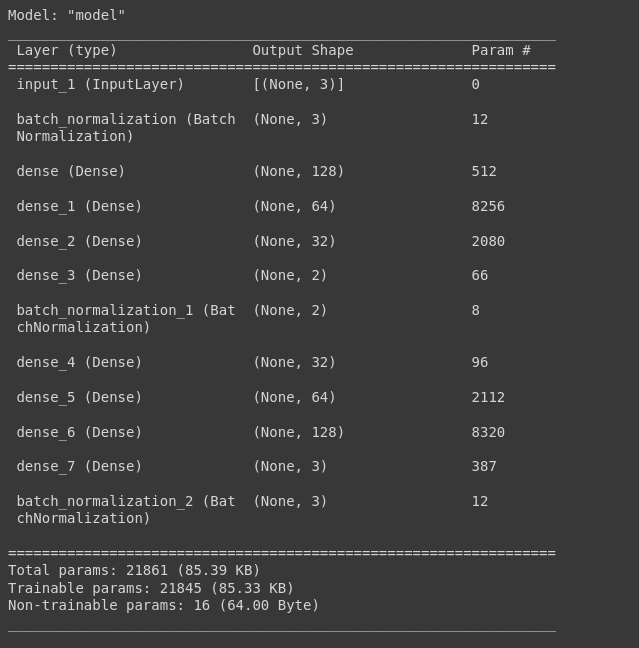
\includegraphics[width=\linewidth]{images/autoencoder_summary.png}
	      		\caption{Autoencoder summary}
	      		\label{fig:autoencoder-summary}
	      	\end{subfigure}
	      	\label{fig:autoencoder}
	      	\caption{Autoencoder structure}
	      \end{figure}
	      
	      \textbf{Experiments with the autoencoders:}
	      \begin{itemize}
	      	\item \textbf{Dimensionality reduction on swiss roll dataset (100k points):}\\
	      	      We again utilized the sklearn's \textit{make\_swiss\_roll} function to create a Swiss roll dataset with 100,000 points. We then used this dataset to train our autoencoder. Since our main goal was to understand the hidden patterns in the data and learn a lower dimensional embedding, we skipped the usual step of dividing the dataset into parts to check the model's performance. We wanted our model to get very good at understanding the specifics of this data, so we let it focus only on learning from it. This straightforward approach helped the model to get better at capturing the unique features of the swiss roll dataset. \\
	      	      We trained this model for 50 epochs without GPU acceleration to mimic a weak computer and to our surprise, we were able to train this model on 100k points in around 10 minutes which can be compared to the datafold's performance on the same dataset size. The loss curve can be seen in figure \ref{fig:autoencoder-training-100k}. We plotted the results for randomly selected 10,000 points for easy visualization as can be seen in figure \ref{fig:autoencoder-result-100k}. The results clearly show some patterns emerging which might be useful in understanding the dynamics of the underlying curve of the swiss roll dataset. The trustworthiness metric is also comparable with the score achieved using datafold.
               \begin{figure}[H]
	      	\centering
	      	\begin{subfigure}{0.45\textwidth}
	      		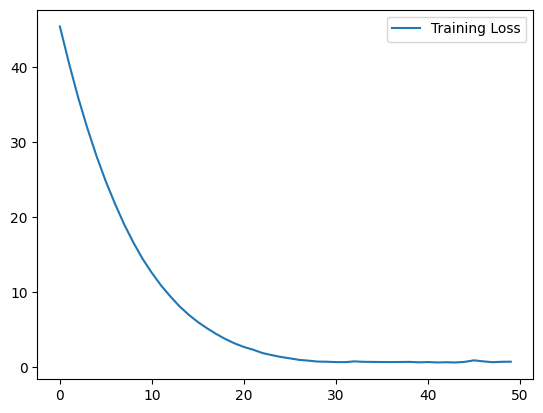
\includegraphics[width=\linewidth]{images/autoencoder_training_100k.png}
	      		\caption{Training Loss curve}
	      		\label{fig:autoencoder-training-100k}
	      	\end{subfigure}
	      	\begin{subfigure}{0.45\textwidth}
	      		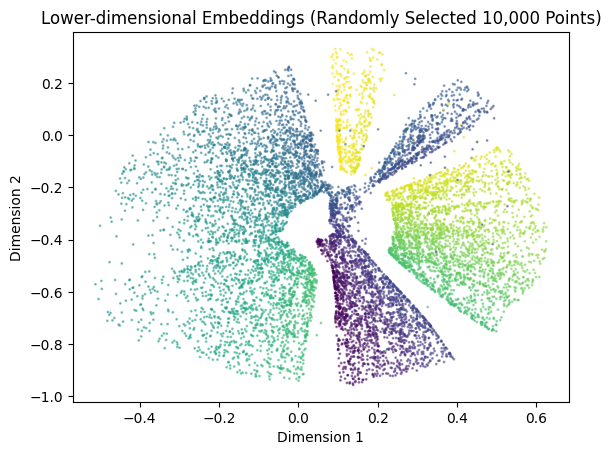
\includegraphics[width=\linewidth]{images/autoencoder_result_100k.png}
	      		\caption{Embedding result}
	      		\label{fig:autoencoder-result-100k}
	      	\end{subfigure}
	      	\label{fig:autoencoder-100k}
	      	\caption{Autoencoder training curve and result on Swiss roll curve for 100,000 points.}
	      \end{figure}

            \item \textbf{Dimensionality reduction on Swiss roll dataset (1 million points):}\\
            We replicated the steps that we used in our previous implementation of the autoencoder on a dataset with 100,00 points, extending our approach to train the autoencoder on an even larger dataset comprising 1 million points. This poses a significant challenge for other libraries and algorithms including Diffusion Maps. \\
            These algorithms often struggle with scalability when dealing with very large datasets as they require extensive computations and memory resources. They face difficulties in efficiently preprocessing and extracting meaningful embeddings from datasets with a million points.\\
            In contrast, our autoencoder implementation showcased robust performance, successfully learning embeddings of the Swiss roll dataset with 1 million points. The autoencoder uses minibatching during its learning process to look at the data and learn the embeddings.  This might be problematic as it might not retain the global relationships within in the data. But, even with these limitations, we are able to learn embeddings on the dataset with a good local trustworthiness metric. Naturally, training the autoencoder on such huge datasets takes time. The loss curve can be seen in figure \ref{fig:autoencoder-training-1M}. The resulting embeddings can be seen in figure \ref{fig:autoencoder-result-1M}.
            \begin{figure}[H]
	      	\centering
	      	\begin{subfigure}{0.45\textwidth}
	      		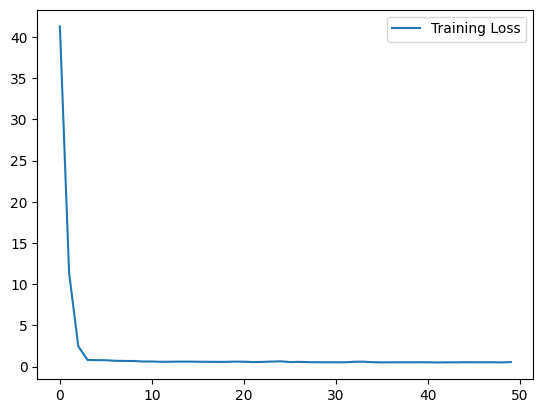
\includegraphics[width=\linewidth]{images/autoencoder_training_1M.png}
	      		\caption{Training Loss curve}
	      		\label{fig:autoencoder-training-1M}
	      	\end{subfigure}
	      	\begin{subfigure}{0.45\textwidth}
	      		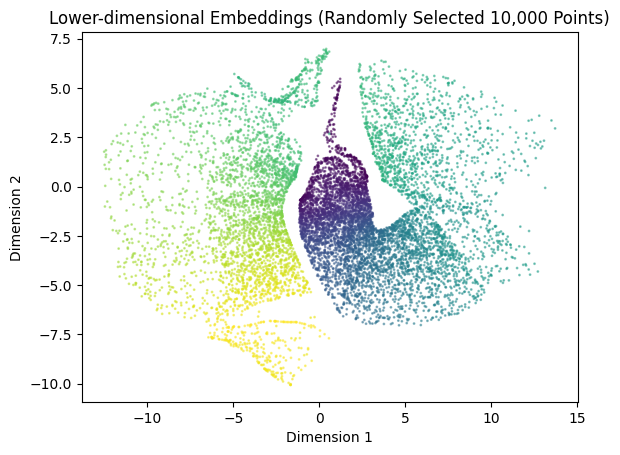
\includegraphics[width=\linewidth]{images/autoencoder_result_1M.png}
	      		\caption{Embedding result}
	      		\label{fig:autoencoder-result-1M}
	      	\end{subfigure}
	      	\label{fig:autoencoder-1M}
	      	\caption{Autoencoder training curve and result on swiss roll curve for 1 million points.}
	      \end{figure}

            \item \textbf{Dimensionality reduction on Google news Word2Vec dataset: }\\
            Having obtained good results on the Swiss Roll Dataset, we decided to use our autoencoder to learn the embeddings on a real-life dataset of Google News Word2Vec dataset consisting of 3 million points each characterized by 300-dimensional features. \\
            To test the efficacy of our model, we only picked a random sample of 100,000 data points and tried to fit our model on this dataset. The training loss curve and results can be seen in figure \ref{fig:autoencoderword2vec}. Although we were able to fit our model on the dataset, the results as seen in Fig. \ref{fig:autoencoder-result-word2vec} are not satisfactory and do not give proper embeddings with only a trustworthiness score of 64\%. \\
            Several factors could be responsible for the subpar performance of our model on this dataset. One potential reason may be insufficient preprocessing of the dataset. Additionally, the complexity and dimensionality of the Google News Word2Vec dataset pose a unique challenge. Inadequate tuning of hyperparameters or model architecture for such high-dimensional data can also hinder the model's capacity to capture relevant patterns effectively. \\
            Further investigation into the specific characteristics of the dataset, experimentation with different preprocessing techniques, and fine-tuning of  model parameters may be necessary to improve the performance on this challenging real-world dataset.

            \begin{figure}[H]
            \centering
            \begin{subfigure}{0.45\textwidth}
                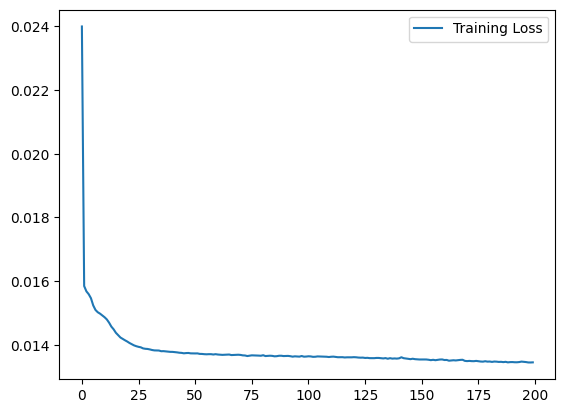
\includegraphics[width=\linewidth]{images/autoencoder_training_word2vec.png}
                \caption{Training Loss curve}
                \label{fig:autoencoder-training-word2vec}
            \end{subfigure}
            \begin{subfigure}{0.45\textwidth}
                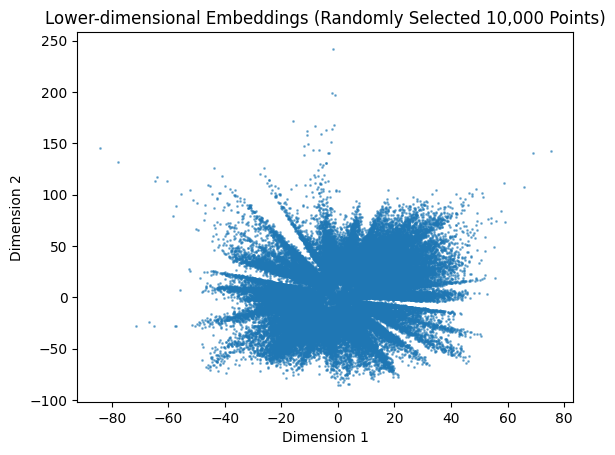
\includegraphics[width=\linewidth]{images/autoencoder_result_word2vec.png}
                \caption{Embedding result}
                \label{fig:autoencoder-result-word2vec}
            \end{subfigure}
            \caption{Autoencoder training curve and result on Google News Word2Vec dataset (100,000 points)}
            \label{fig:autoencoderword2vec}
        \end{figure}

        
        \end{itemize}
            
\end{itemize}